\documentclass{standalone}
\usepackage{tikz}
\usetikzlibrary{patterns, positioning}


\begin{document}
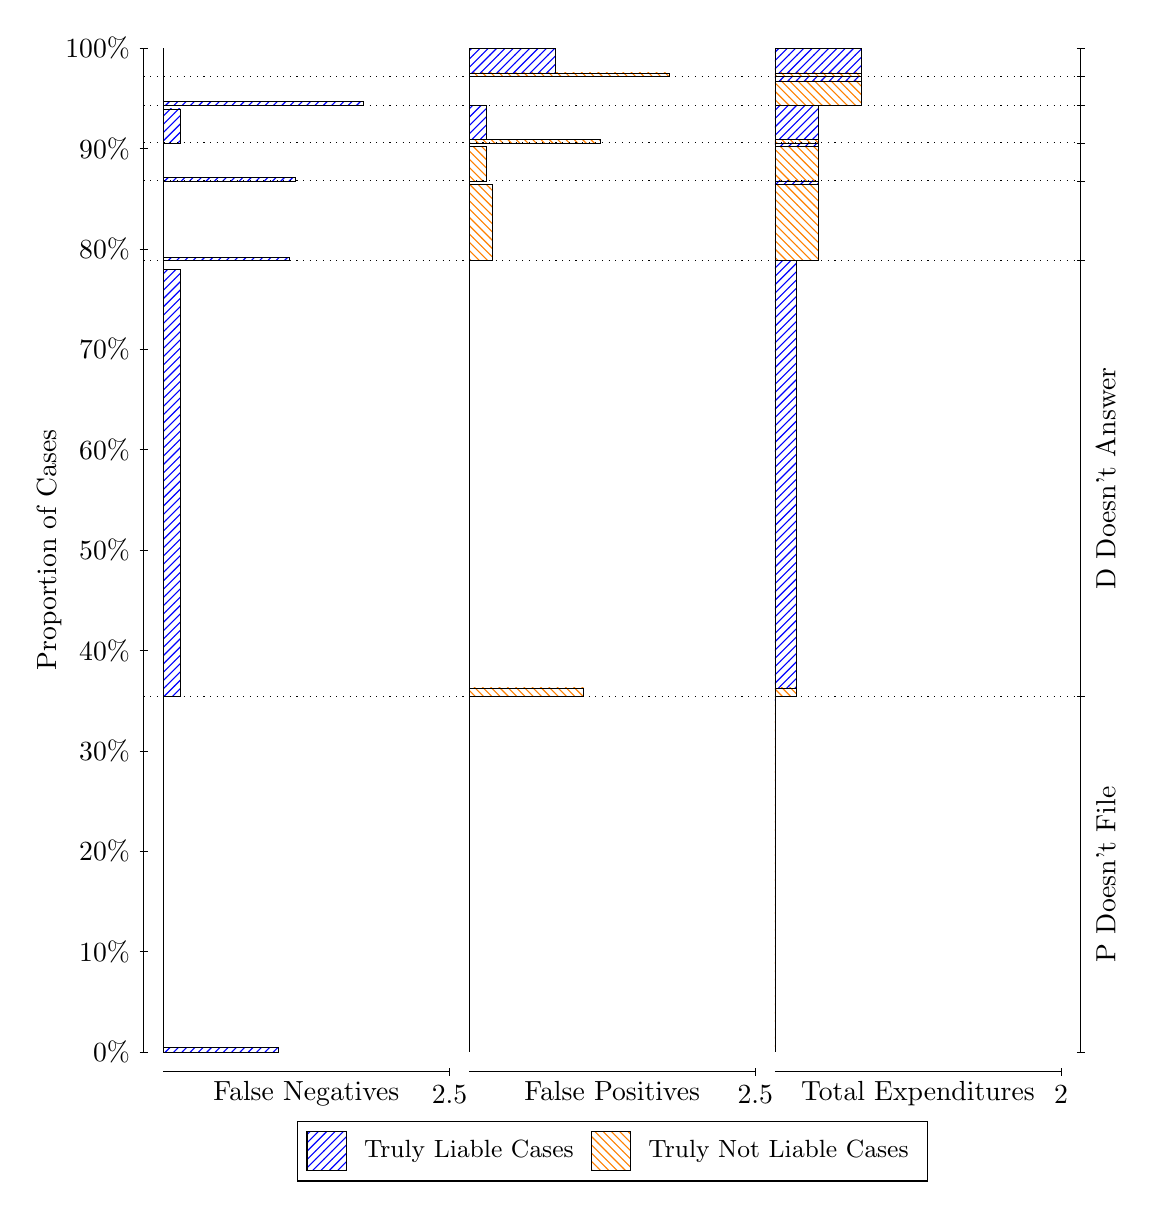
\begin{tikzpicture}
\draw[black, very thin] (1.5,1.75) -- (1.5,14.5);
\node[rotate=90, text=black, anchor=center] at (0.3, 8.125) {Proportion of Cases};
\draw[black, very thin] (1.45,1.75) -- (1.55,1.75);
\node[text=black, anchor=east] at (1.45, 1.75) {0\%};
\draw[black, very thin] (1.45,3.025) -- (1.55,3.025);
\node[text=black, anchor=east] at (1.45, 3.025) {10\%};
\draw[black, very thin] (1.45,4.3) -- (1.55,4.3);
\node[text=black, anchor=east] at (1.45, 4.3) {20\%};
\draw[black, very thin] (1.45,5.575) -- (1.55,5.575);
\node[text=black, anchor=east] at (1.45, 5.575) {30\%};
\draw[black, very thin] (1.45,6.85) -- (1.55,6.85);
\node[text=black, anchor=east] at (1.45, 6.85) {40\%};
\draw[black, very thin] (1.45,8.125) -- (1.55,8.125);
\node[text=black, anchor=east] at (1.45, 8.125) {50\%};
\draw[black, very thin] (1.45,9.4) -- (1.55,9.4);
\node[text=black, anchor=east] at (1.45, 9.4) {60\%};
\draw[black, very thin] (1.45,10.675) -- (1.55,10.675);
\node[text=black, anchor=east] at (1.45, 10.675) {70\%};
\draw[black, very thin] (1.45,11.95) -- (1.55,11.95);
\node[text=black, anchor=east] at (1.45, 11.95) {80\%};
\draw[black, very thin] (1.45,13.225) -- (1.55,13.225);
\node[text=black, anchor=east] at (1.45, 13.225) {90\%};
\draw[black, very thin] (1.45,14.5) -- (1.55,14.5);
\node[text=black, anchor=east] at (1.45, 14.5) {100\%};

\draw[black, very thin] (13.4,1.75) -- (13.4,14.5);
\draw[black, very thin] (13.35,1.75) -- (13.45,1.75);
\node[anchor=west] at (13.35, 1.75) {};
\draw[black, very thin] (13.35,6.2649) -- (13.45,6.2649);
\node[anchor=west] at (13.35, 6.2649) {};
\draw[black, very thin] (13.35,11.8) -- (13.45,11.8);
\node[anchor=west] at (13.35, 11.8) {};
\draw[black, very thin] (13.35,12.814) -- (13.45,12.814);
\node[anchor=west] at (13.35, 12.814) {};
\draw[black, very thin] (13.35,13.296) -- (13.45,13.296);
\node[anchor=west] at (13.35, 13.296) {};
\draw[black, very thin] (13.35,13.773) -- (13.45,13.773);
\node[anchor=west] at (13.35, 13.773) {};
\draw[black, very thin] (13.35,14.135) -- (13.45,14.135);
\node[anchor=west] at (13.35, 14.135) {};
\draw[black, very thin] (13.35,14.5) -- (13.45,14.5);
\node[anchor=west] at (13.35, 14.5) {};

\draw[black, very thin, pattern color=blue, pattern=north east lines] (1.75,1.75) rectangle (3.2033,1.8102);
\draw[black, very thin, pattern color=orange, pattern=north west lines] (1.75,1.8102) rectangle (1.75,6.2649);
\draw[black, very thin, pattern color=blue, pattern=north east lines] (1.75,6.2649) rectangle (1.968,11.692);
\draw[black, very thin, pattern color=orange, pattern=north west lines] (1.75,11.692) rectangle (1.75,11.8);
\draw[black, very thin, pattern color=blue, pattern=north east lines] (1.75,11.8) rectangle (3.3487,11.845);
\draw[black, very thin, pattern color=orange, pattern=north west lines] (1.75,11.845) rectangle (1.75,12.814);
\draw[black, very thin, pattern color=blue, pattern=north east lines] (1.75,12.814) rectangle (3.4213,12.861);
\draw[black, very thin, pattern color=orange, pattern=north west lines] (1.75,12.861) rectangle (1.75,13.296);
\draw[black, very thin, pattern color=blue, pattern=north east lines] (1.75,13.296) rectangle (1.968,13.728);
\draw[black, very thin, pattern color=orange, pattern=north west lines] (1.75,13.728) rectangle (1.75,13.773);
\draw[black, very thin, pattern color=blue, pattern=north east lines] (1.75,13.773) rectangle (4.2933,13.824);
\draw[black, very thin, pattern color=orange, pattern=north west lines] (1.75,13.824) rectangle (1.75,14.135);
\draw[black, very thin, pattern color=orange, pattern=north west lines] (1.75,14.135) rectangle (1.75,14.185);
\draw[black, very thin, pattern color=blue, pattern=north east lines] (1.75,14.185) rectangle (1.75,14.5);
\draw[black, very thin, pattern color=orange, pattern=north west lines] (5.6333,1.75) rectangle (5.6333,6.2047);
\draw[black, very thin, pattern color=blue, pattern=north east lines] (5.6333,6.2047) rectangle (5.6333,6.2649);
\draw[black, very thin, pattern color=orange, pattern=north west lines] (5.6333,6.2649) rectangle (7.0867,6.3735);
\draw[black, very thin, pattern color=blue, pattern=north east lines] (5.6333,6.3735) rectangle (5.6333,11.8);
\draw[black, very thin, pattern color=orange, pattern=north west lines] (5.6333,11.8) rectangle (5.924,12.77);
\draw[black, very thin, pattern color=blue, pattern=north east lines] (5.6333,12.77) rectangle (5.6333,12.814);
\draw[black, very thin, pattern color=orange, pattern=north west lines] (5.6333,12.814) rectangle (5.8513,13.249);
\draw[black, very thin, pattern color=blue, pattern=north east lines] (5.6333,13.249) rectangle (5.6333,13.296);
\draw[black, very thin, pattern color=orange, pattern=north west lines] (5.6333,13.296) rectangle (7.3047,13.341);
\draw[black, very thin, pattern color=blue, pattern=north east lines] (5.6333,13.341) rectangle (5.8513,13.773);
\draw[black, very thin, pattern color=orange, pattern=north west lines] (5.6333,13.773) rectangle (5.6333,14.084);
\draw[black, very thin, pattern color=blue, pattern=north east lines] (5.6333,14.084) rectangle (5.6333,14.135);
\draw[black, very thin, pattern color=orange, pattern=north west lines] (5.6333,14.135) rectangle (8.1767,14.185);
\draw[black, very thin, pattern color=blue, pattern=north east lines] (5.6333,14.185) rectangle (6.7233,14.5);
\draw[black, very thin, pattern color=orange, pattern=north west lines] (9.5167,1.75) rectangle (9.5167,6.2047);
\draw[black, very thin, pattern color=blue, pattern=north east lines] (9.5167,6.2047) rectangle (9.5167,6.2649);
\draw[black, very thin, pattern color=orange, pattern=north west lines] (9.5167,6.2649) rectangle (9.7892,6.3735);
\draw[black, very thin, pattern color=blue, pattern=north east lines] (9.5167,6.3735) rectangle (9.7892,11.8);
\draw[black, very thin, pattern color=orange, pattern=north west lines] (9.5167,11.8) rectangle (10.062,12.77);
\draw[black, very thin, pattern color=blue, pattern=north east lines] (9.5167,12.77) rectangle (10.062,12.814);
\draw[black, very thin, pattern color=orange, pattern=north west lines] (9.5167,12.814) rectangle (10.062,13.249);
\draw[black, very thin, pattern color=blue, pattern=north east lines] (9.5167,13.249) rectangle (10.062,13.296);
\draw[black, very thin, pattern color=orange, pattern=north west lines] (9.5167,13.296) rectangle (10.062,13.341);
\draw[black, very thin, pattern color=blue, pattern=north east lines] (9.5167,13.341) rectangle (10.062,13.773);
\draw[black, very thin, pattern color=orange, pattern=north west lines] (9.5167,13.773) rectangle (10.607,14.084);
\draw[black, very thin, pattern color=blue, pattern=north east lines] (9.5167,14.084) rectangle (10.607,14.135);
\draw[black, very thin, pattern color=orange, pattern=north west lines] (9.5167,14.135) rectangle (10.607,14.185);
\draw[black, very thin, pattern color=blue, pattern=north east lines] (9.5167,14.185) rectangle (10.607,14.5);
\draw[black, dotted] (1.5,6.2649) -- (13.4,6.2649);
\draw[black, dotted] (1.5,11.8) -- (13.4,11.8);
\draw[black, dotted] (1.5,12.814) -- (13.4,12.814);
\draw[black, dotted] (1.5,13.296) -- (13.4,13.296);
\draw[black, dotted] (1.5,13.773) -- (13.4,13.773);
\draw[black, dotted] (1.5,14.135) -- (13.4,14.135);
\draw[black, very thin] (1.75,1.5) -- (5.3833,1.5);
\node[text=black, anchor=north] at (3.5667, 1.5) {False Negatives};
\draw[black, very thin] (5.3833,1.45) -- (5.3833,1.55);
\node[text=black, anchor=north] at (5.3833, 1.45) {2.5};

\draw[black, very thin] (5.6333,1.5) -- (9.2667,1.5);
\node[text=black, anchor=north] at (7.45, 1.5) {False Positives};
\draw[black, very thin] (9.2667,1.45) -- (9.2667,1.55);
\node[text=black, anchor=north] at (9.2667, 1.45) {2.5};

\draw[black, very thin] (9.5167,1.5) -- (13.15,1.5);
\node[text=black, anchor=north] at (11.333, 1.5) {Total Expenditures};
\draw[black, very thin] (13.15,1.45) -- (13.15,1.55);
\node[text=black, anchor=north] at (13.15, 1.45) {2};

\node[text=black, centered, rotate=90] at (13.72, 4.0075) {P Doesn't File};
\node[text=black, centered, rotate=90] at (13.72, 9.0327) {D Doesn't Answer};






\draw (7.449999999999999,1.5) node[draw=none] (baseCoordinate) {};
\begin{scope}[align=center]
        \matrix[scale=0.5, draw=black, below=0.5cm of baseCoordinate, nodes={draw}, column sep=0.1cm]{
            \node[rectangle, draw, minimum width=0.5cm, minimum height=0.5cm, pattern color=blue, pattern=north east lines] {}; &
            \node[draw=none, font=\small, text=black] (B) {Truly Liable Cases}; &
            \node[rectangle, draw, minimum width=0.5cm, minimum height=0.5cm, pattern color=orange, pattern=north west lines] {}; &
            \node[draw=none, font=\small, text=black] (B) {Truly Not Liable Cases}; \\
            };
\end{scope}

\end{tikzpicture}
\end{document}